\chapter{Morphologischer Kasten (Ali)}
Als Hilfsmittel zur Konzeptfindung, haben wir uns dazu entschieden einen Morphologischen Kasten für die Drohne und für die Lastaufhängung zu erstellen.
Die Funktion unserer Drohne und der Lastaufhängung werden in Anlehnung an die Anforderungsliste in Teilfunktionen aufgespalten. Zu diesen Teilfunktion werden dann physikalische Wirkprinzipien gefunden und in einer Matrix notiert, dem sogenannten Morphologischen Kasten. Aus diesen Wirkprinzipien entstehen dann Wirkstrukturen, welche dann anhand von technischen und wirtschaftlichen Kriterien bewertet werden. Hier weicht unsere Konzeptionsmethoden vom klassischen Morphologischen Kasten ab, da wir auf eine ausführliche wirtschaftliche Bewertung verzichten. Das Wirkprinzip mit der höchsten relativen Wertung wird dann eventuell mit anderen hochbewerteten Wirkprinzipien ergänzt und bildet dann die Grundlage für unser Gesammtkonzept. 

\section{Drohne}
Wie in Abb \ref{fig:Morphologischer-Kasten-Drohne} gezeigt haben wir unsere Drohne anhand der Anforderungsliste in Teilaufgaben unterteilt und diese verallgemeinert. Für die Aufgaben suchen wir im Team nach Lösungsanzätzen und Wirkprinzipien. Es werden sämtliche Ideen festgehalten ohne vorzeitige Bewertungen.
So wird auch der Vorschlag Holz als mögliches Material aus dem Teile der Drohne hergestellt werden können, wahrgenommen.
% sich für das Material aus dem Teile der Drohne bestehen sollen auch Lösungen wie Holz  

\begin{figure}[h]
	\centering
	\includegraphics[width=1.00\textwidth]
	{bilder/Morphologischer_Kasten/MorphKastDrohne}
	\caption{Morphologischer-Kasten-Drohne}
	%{Beschädigter Stabilisator\cite{Aerossurance}} 
	\label{fig:Morphologischer-Kasten-Drohne}
\end{figure}

Anschließend suchen wir nach Wirkstrukturen. Dabei beachten wir das sich die unterschiedlichen Wirkprinzipien einer Wirkstrucktur auch vertragen. Holz zum Beispiel können wir nicht 3D-Drucken. in der Abbildung sind unsere drei Wirkstrukturen zu sehen.

%\begin{figure}[H]
%	\centering
%	\includegraphics[width= 0.40\textwidth]{Bilder/MorphKastDrohne.jpg}
%	\caption[Beschädigter horizontaler Stabilisator]{Beschädigter Stabilisator %\cite{Aerossurance}} 
%	\label{fig:Morphologischer-Kasten-Drohne}
%\end{figure}


\subsection{Technische Bewertung}
Bei der technischen Bewertung wird den drei Wirkstrukturen eine relative Wertigkeit zugeordnet. Eine wirtschaftliche Bewertung wird hier nicht durchgeführt. Einige wirtschaftliche Aspekte werden trotzdem berücksichtigt. So zum Beispiel das die Materialien weitestgehend an der Thi schon verfügbar sein sollten und nicht nachbestellt werden müssen. Ein weiteres wirtschaftliches Kriterium ist, dass wir unsere Fertigungsteile nach Möglichkeit entweder selbst oder in einer der Werkstätten an der THI fertigen können und dementsprechend keine außerhochschulischen Dienste in Anspruch nehmen müssen.
Weitere Kriterien orientieren sich eher an den Vorstellungen die wir an das Projekt haben. So ist eines unserer Ziele eine möglichst leichte und kompakte Drohne zu entwickeln und trotzdem soll sie robust sein.  Ebenfals ist es uns wichtig möglichst viel selbst herstellen zu können und unsere Arbeit innovativ zu gestalten. Dementsprechend sind die Gewichtungen der Kriterien recht subjektiv. Die Kriterien werden mit eins (unwichtig bzw. vorgegeben) bis vier(sehr wichtig) gewichtet. Jede Wirkstruktur wir unabhängig von den anderen Wirkstrukturen bewertet. Schlißlich werden die Bewertungen aufsummiert und durch die maximal erreichbare Bewertung geteilt sogass sich eine relative Bewertung ergibt. Wie in Abbildung zu sehen hat die 1.Wirkstruktur "Alpha" die höchste relative Wertigkeit und ist somit Grundlage für unser endgültiges Konzept.
\begin{figure}[h!]
	\centering
	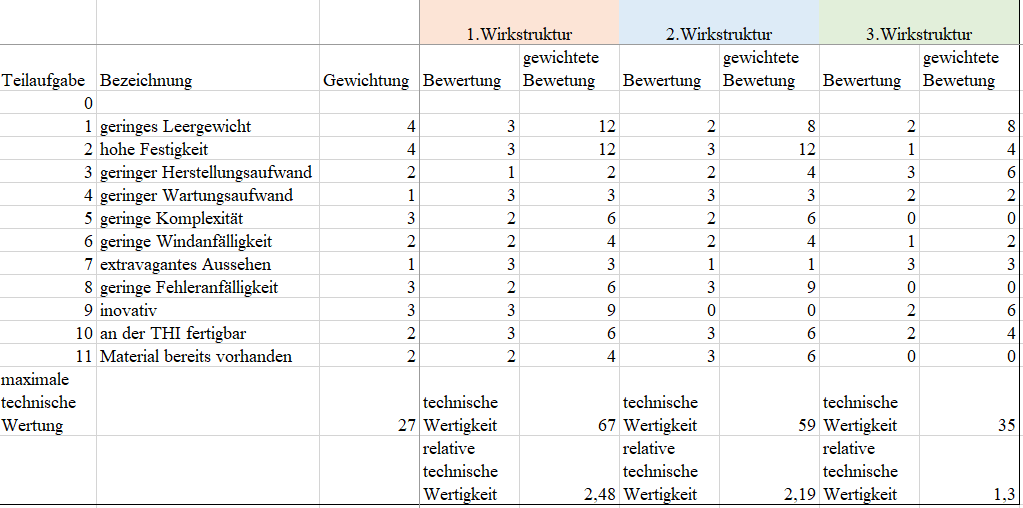
\includegraphics[width= 1.00\textwidth]{bilder/Morphologischer_Kasten/BewDrohne}
	\caption{Technische-Bewertung-Drohne}
	%{Beschädigter Stabilisator\cite{Aerossurance}} 
	%	\label{fig:Morphologischer-Kasten-Drohne}
\end{figure}

\subsection{Stärkendiagramm}



\section{Lastaufhängung}
Für den Morphologischen Kasten der Lastaufhängung wird der gleiche Prozess wie bereits in den Punkten weiter oben beschrieben, angewendet.
Die Überfunktion Lastaufhängung wird in Teilfunktionen aufgeteilt. In Abbildung ist zu erkennen wie für jede Teilaufgabe mindestens drei Lösungselemente gefunden wurden. Im darauffolgenden Schritt werden diese Wirkprinzipien zu Wirkstrukturen verheiratet.
\begin{figure}[h!]
	\centering
	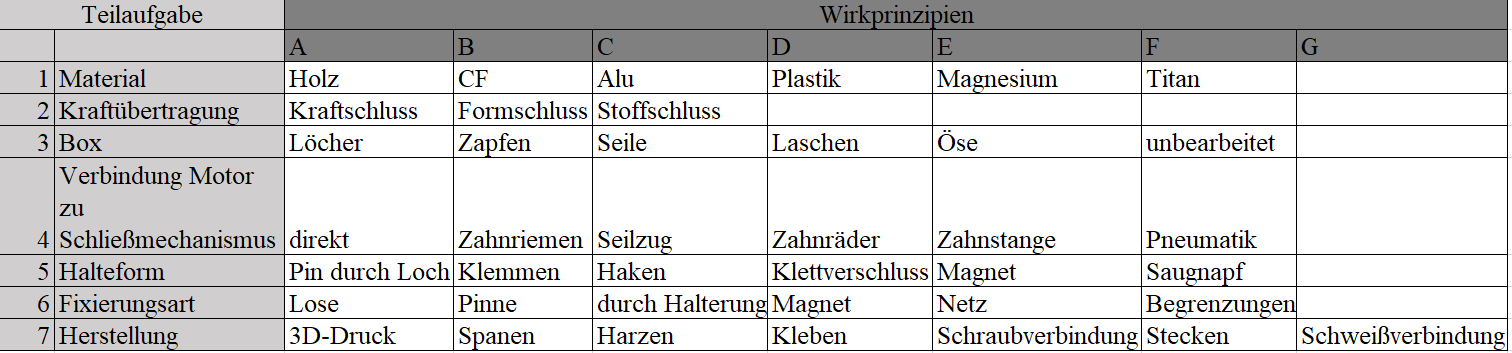
\includegraphics[width= 1.00\textwidth]{bilder/Morphologischer_Kasten/MorphKastLastaufh}
	\caption{Morphologischer-Kasten-Lastaufhaengung}
	%{Beschädigter Stabilisator\cite{Aerossurance}} 
	%	\label{fig:Morphologischer-Kasten-Drohne}
\end{figure}

\subsection{Technische Bewertung}

\begin{figure}[h!]
	\centering
	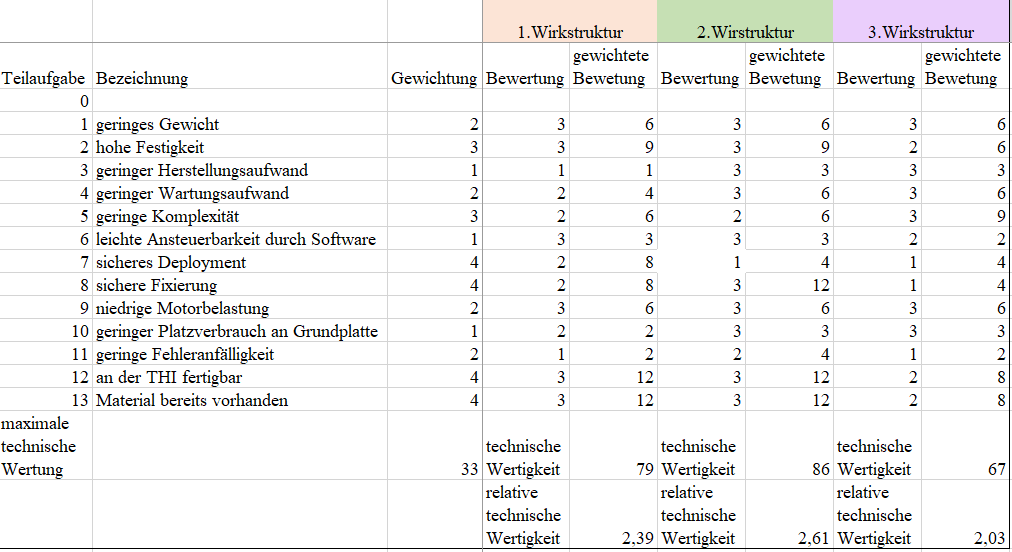
\includegraphics[width= 1.00\textwidth]{bilder/Morphologischer_Kasten/BewLastaufh}
	\caption{Technische-Bewertung-Lastaufhaengung}
	%{Beschädigter Stabilisator\cite{Aerossurance}} 
	%	\label{fig:Morphologischer-Kasten-Drohne}
\end{figure}

\subsection{Stärkendiagramm}


\section{Konzeptauswahl}